\chapter{Architektura systemu}
\label{Chapter5}

\begin{figure}[H] 
\centering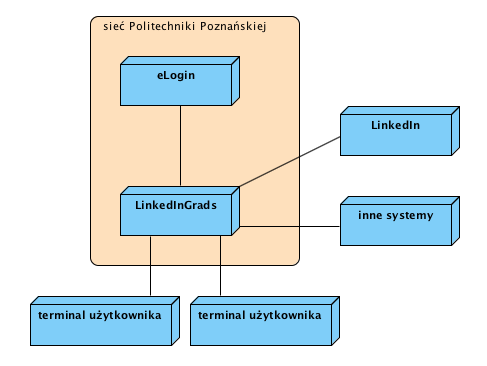
\includegraphics[width=15cm]{figures/image2}
\caption{Architektura systemu LinkedInGrads}\label{rys:use-case-diagram}
\end{figure}

W rozdziale przedstawione zostaną zagadnienia związane z architekturą systemu LinkedInGrads. Ukazane zostaną zastosowane podejścia architektoniczne, podjęte decyzje (razem z ich uzasadnieniami oraz zależnościami), zobrazowany będzie przyjęty schemat bazy danych. W celu lepszego przedstawienia tematu architektury, ze względu na jego złożoność, w podrozdziale 5.4. Perspektywy architektoniczne wykorzystano model 4+1 Views.

\section{Zastosowane podejście architektoniczne}
\label{Chapter52}

Rozdział dotyczy wzorca projektowego, w oparciu o który zaprojektowano architekturę systemu.

\subsection{Architektura MVC}

Wzorzec projektowy, który wykorzystano w systemie to MVC (ang. Model View Controller). Pozwala on na organizację aplikacji posiadających interfejs użytkownika dzieląc kod na trzy główne części przedstawione na diagramie poniżej. Dzięki takimi rozwiązaniu można odseparować wewnętrzną reprezentację informacji od sposobu jej prezentacji użytkownikowi końcowemu.

\begin{figure}[H] 
\centering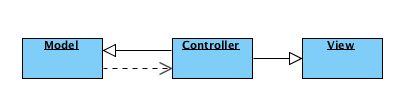
\includegraphics[width=15cm]{figures/image3}
\caption{Zależności warstw w architekturze MVC}\label{rys:use-case-diagram}
\end{figure}

Zgodnie z rysunkiem 5.2. występuje podział aplikacji na:

\begin{itemize}
\item Model - warstwa reprezentująca logikę biznesową aplikacji, odpowiada również za stan aplikacji oraz utrzymywanie informacji,
\item Controller - warstwa odpowiedzialna za komunikację i sterowanie, przyjmuje żądania użytkownika, reagując na nie aktualizacją modeli, prezentuje informacje modeli używając do tego celu widoków,
\item View - warstwa prezentująca dane i interfejs użytkownikowi, nie zajmuje się przetwarzaniem informacji.
\end{itemize}

Powyższy wzorzec posiada wiele zalet. Jedną z nich może być bardzo czytelny podział odpowiedzialności poszczególnych części aplikacji, który znacznie obniża barierę wejścia w razie dołączenia nowego członka do projektu. Główne korzyści płyną jednak z faktu odseparowania modeli, czyli logiki biznesowej od pozostałych warstw: widoków oraz kontrolerów. Wykorzystanie samodzielnych modeli: 

\begin{itemize}
\item sprawia, że mogą być użyte ponownie w wielu miejscach, niezależnie od interfejsów, Przykładem może być prezentowanie danych z tego samego modelu w różnych formatach, wykorzystując do tego różne widoki
\item upraszcza testowanie kodu logiki biznesowej, która nie jest powiązane z warstwami wymuszającymi np. wytwarzanie żądania http
\item ułatwia rozbudowę interfejsów, przy solidnie zbudowanej logice, najczęściej wykonywane zmiany: dodawanie nowych i modyfikowanie istniejących widoków nie wpływa wcale na główną część systemu
\item minimalizuje sposobność naruszenia reguł biznesowych, ponieważ wyłącznie model może modyfikować dane
\end{itemize}

Wadą tego wzorca są kosztowne zmiany interfejsów już istniejących modeli. W przypadku powiązania wielu widoków z danym modelem, należy zadbać o stosowne zmiany w każdym z nich. Dodatkowo, testowanie złożonych widoków, korzystających z wielu modeli może okazać się bardzo trudne, ze względu na liczbę powiązanych różnych obiektów.

\subsection{Podział warstwy Model oraz ReportRenderes}

Na rysunku 5.3 przedstawiono podział warstw wzorca Model View Controller oraz wprowadzone modyfikacje:

\begin{figure}[H] 
\centering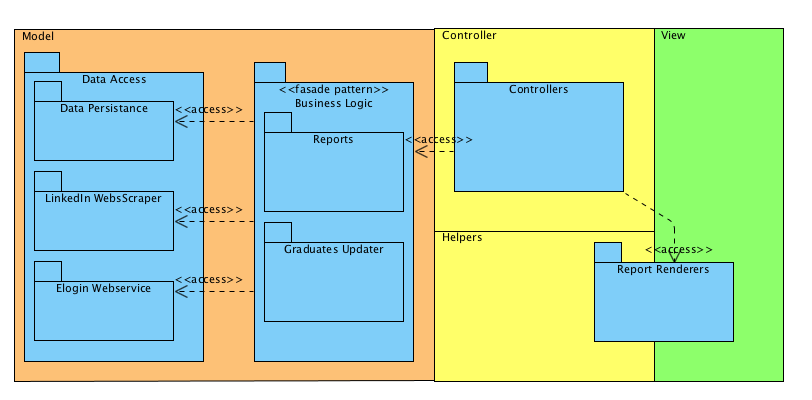
\includegraphics[width=15cm]{figures/image4}
\caption{Architektura MVC w systemie LinkedInGrads}\label{rys:use-case-diagram}
\end{figure}

Dokonano podziału warstwy odpowiadającej za logikę - model - na dwie dodatkowe warstwy:

\begin{itemize}
\item Business Logic - odpowiada za implementację właściwych reguł biznesowych oraz obiektów,
\item Data Access - odpowiada za komunikację z bazą danych: odczyt oraz zapis, interakcję z zewnętrznymi źródłami danych, co jest wynikiem komunikacji z klasami warstw Business Logic.
\end{itemize}

Rozwiązanie takie oprócz zwiększenia czytelności podziału odpowiedzialności powoduje zwiększenie bezpieczeństwa zachowania reguł biznesowych - nic poza warstwą Business Logic nie powinno wykonywać zleceń do warstwy Data Access i tym samym mieć możliwości modyfikowania danych. Odizolowanie logiki od warstwy odpowiadającej za komunikację z bazą danych sprawia, że ewentualna zmiana silnika bazy danych na inny, powinna przebiegać szybko i nie spowoduje olbrzymiego nakładu czasowego.

W obrębie klasy Business Logic zastosowano fasadę, ułatwiającą korzystanie z Raportów. Zgodnie z diagramem utworzono warstwę ReportRenderers, odpowiedzialną za generowanie raportów w oczekiwanych formatach - wykazuje więc cechy warstwy View, dostarcza odpowiednio zaprezentowane dane. ReportRenderes inspirowana była wzorcami Visitor oraz Builder, jest wykorzystywana przez kontrolery i wizytuje obiekty Report. Rozwiązanie takie pozwala na elastyczne zarządzanie dostępnymi formatami raportów.

\subsection{Rozbudowa oprogramowania}

Opisane wcześniej rozwiązania sprawiają, że zwiększa się stopień odizolowania właściwej logiki biznesowej. Pozwala to na używanie warstwy Model, a nawet samej Business Logic przez inne zewnętrzne moduły, które stają się w stosunku do niej klientami. Dodatkowo organizacja generowania raportów oparta o znane wzorce projektowe, sprawia, że rozbudowa o nowe raporty czy też rozszerzenia jest bardzo elastyczna, a ogólna rozbudowa nie będzie kosztowna.

\section{Perspektywy architektoniczne}

Podstawa organizacyjna każdego systemu reprezentowana jest przez elementy strukturalne, zachowanie elementów i kompozycję zarówno jednych jak i drugich. Podzbiory te są dyktowane przez szczególne cechy np. wymagania. Architektura oznacza więc różne zapotrzebowania różnych interesariuszy. Model 4+1, zaprezentowany w kolejnych podrozdziałach wychodzi temu naprzeciw organizując architekturę względem indywidualnych potrzeb grup osób zaangażowanych.

\subsection{Perspektywa logiczna}

Perspektywa logiczna zajmuje się funkcjonalnościami systemu, jakie ma do zaoferowania użytkownikom końcowym. Koncentruje się na operacjach możliwych do zrealizowania i danych.

\begin{figure}[H] 
\centering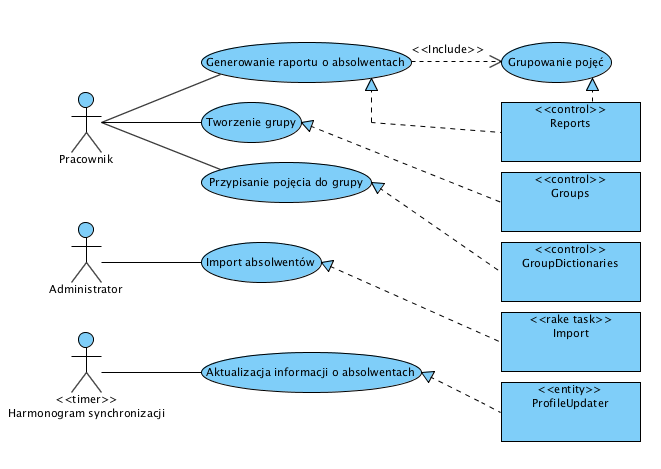
\includegraphics[width=15cm]{figures/image5}
\caption{Perspektywa logiczna}\label{rys:use-case-diagram}
\end{figure}

Na rysunku 5.4. zaprezentowano realizację przypadków użycia przez poszczególne pogrupowane odpowiednio jednostki kodu. Z uwagi na to, że system oparty jest o wzorzec MVC większa część modułów realizujących przypadki użycia to kontrolery. Inaczej jest w przypadku “Importu absolwentów”, który wykonywany jest przez administratora nie przez interfejs aplikacji internetowej, a także “Aktualizacji informacji o absolwentach” wykonywanego w tle, przez sam system.
Dane przedstawione są w rozdziale 5.7. za pomocą schematu związków-encji.

\subsection{Perspektywa implementacyjna}

Perspektywa implementacyjna przedstawia komponenty składające się na system, skupiając się na organizacji modułów i zależnościach między nimi. O ile perspektywa logiczna jest na poziomie pojęciowym, ta perspektywa przedstawia rzeczywiste jednostki, odzwierciedlone w kodzie źródłowym. Przydatna może być podczas konfiguracji, rozwijania oraz konserwacji oprogramowania przez programistów.

\begin{figure}[H] 
\centering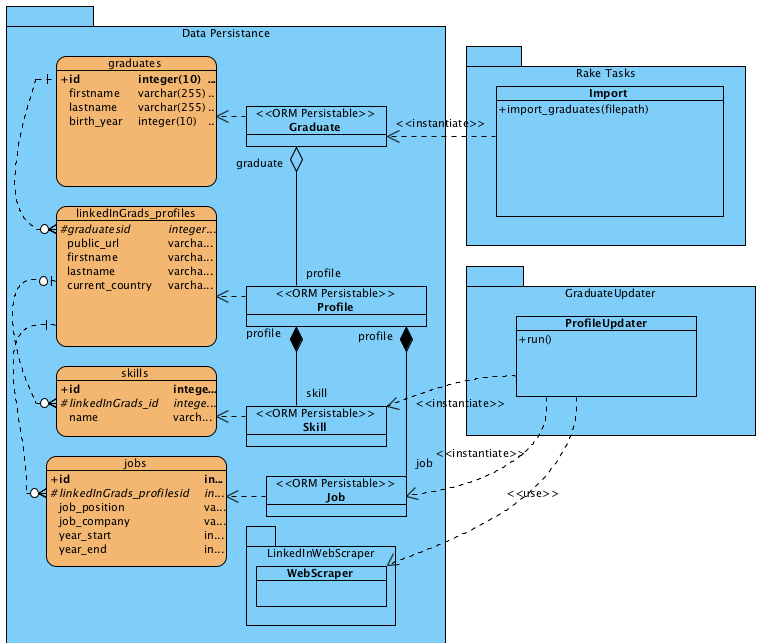
\includegraphics[width=15cm]{figures/image6}
\caption{Perspektywa implementacyjna}\label{rys:use-case-diagram}
\end{figure}

Rysunek 5.5. opisuje możliwe sposoby wypełniania bazy danych danymi. Źródłem danych początkowych jest wykonanie Importu, co powoduje dodanie nowych absolwentów reprezentowanych przez model Graduate. Użycie klasy ProfileUpdater natomiast jest źródłem danych z serwisów zewnętrznych - używa w tym celu LinkedinWebScrapera i inicjalizuje modele Skill oraz Job. Na diagramie pokazano także podstawowe relacje dotyczące raportów oraz ich mapowanie na odpowiadające klasy ORM.

\begin{figure}[H] 
\centering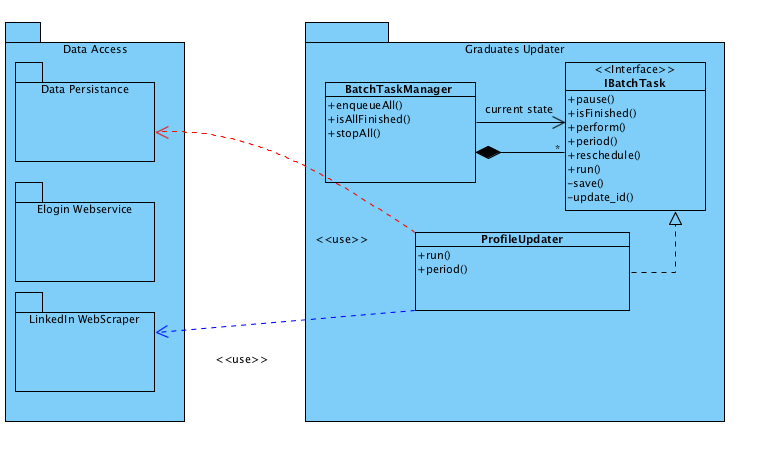
\includegraphics[width=15cm]{figures/image7}
\caption{Diagram klas - menadżer zadań}\label{rys:use-case-diagram}
\end{figure}

Rysunek 5.6. przedstawia realizację menadżera zadań, za którego pomocą istnieje możliwość tworzenia okresowych zadań do wykonania. Zadania te można wstrzymywać oraz wznawiać w dowolnym okresie. Możliwe jest kolejkowanie kilku obiektów klas implementujących interfejs IBatchTask. Procesy mogą być kontrolowane przez menadżera. Wykorzystanie komponentu Batch skupia się wokół aktualizacji danych z serwisów zewnętrznych, które może być długotrwałe, dlatego korzystne jest wykonywanie tego typu zadań w tle.

\begin{figure}[H] 
\centering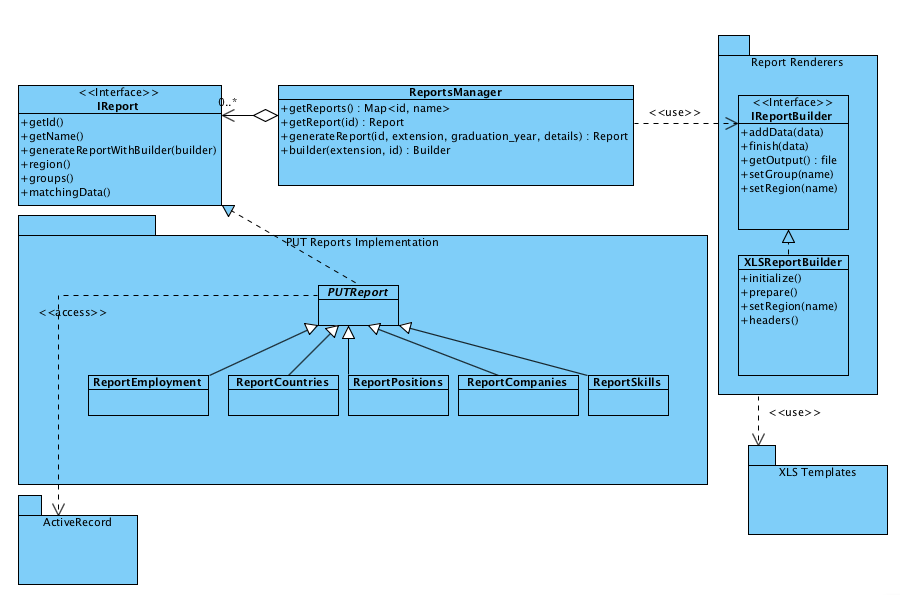
\includegraphics[width=15cm]{figures/image8}
\caption{Diagram klas - generowanie raportów}\label{rys:use-case-diagram}
\end{figure}

Rysunek 5.7. obrazuje logikę biznesową związaną z generowaniem raportów. Podejście inspirowane jest wzorcami projektowymi Visitor oraz Builder. Klasy odpowiedzialne za właściwe dostarczenie danych i generację raportu to klasy implementujące interfejs IReport. Generacja przebiega za pomocą wizytującego obiektu IReportBuilder. Klasy implementujące ten interfejs odpowiedzialne są za różne typy formatów wyjściowych.

\subsection{Perspektywa fizyczna}

Perspektywa fizyczna skupia się na topologii sprzętowej systemu informatycznego służącego do uruchomienia aplikacji. Procesy i zadania mapowane są do elementów na których się wykonują. Informacje mogą być przydatne w szczególności dla osób odpowiedzialnych za wdrożenie systemu lub administratorów. 

Rysunek 5.8. przedstawia rozmieszczenie fizycznych elementów systemu. Mimo tego, że serwer ciągłej integracji oraz baza danych rozlokowane są na jednej maszynie nie ma takiej konieczności, można je umieścić na osobnych serwerach, jeżeli zaistnieje taka potrzeba. Technologie widoczne na rysunku zostały opisane w rozdziale 5.5.

\begin{figure}[H] 
\centering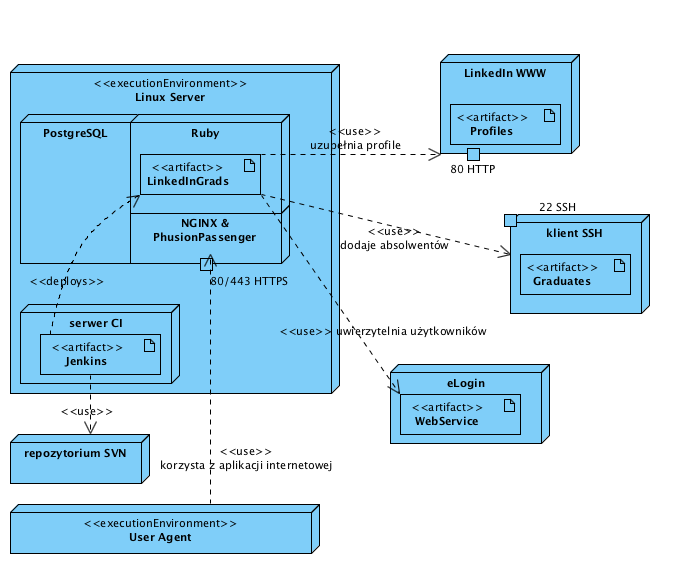
\includegraphics[width=15cm]{figures/image9}
\caption{Perspektywa fizyczna}\label{rys:use-case-diagram}
\end{figure}

\subsection{Perspektywa procesu}

Perspektywa procesu zajmuje się dynamicznym aspektem systemu, wyjaśnia komunikację procesów systemu. Adresuje współbieżność, integrację, wydajność i skalowalność.

Aplikacja LinkedInGrads będąc aplikacją internetową korzysta z protokołu request-response jakim jest HTTP. Cała komunikacja odbywa się więc przez kolejne wiadomości żądań oraz odpowiedzi, co oznacza, że serwer nie wymaga utrzymywania połączeń z klientami.

Rysunek 5.9. obrazuje dynamikę generowania raportów z użyciem pakietu Reports, o którym była mowa także w rozdziale 5.4.2.

\begin{figure}[H] 
\centering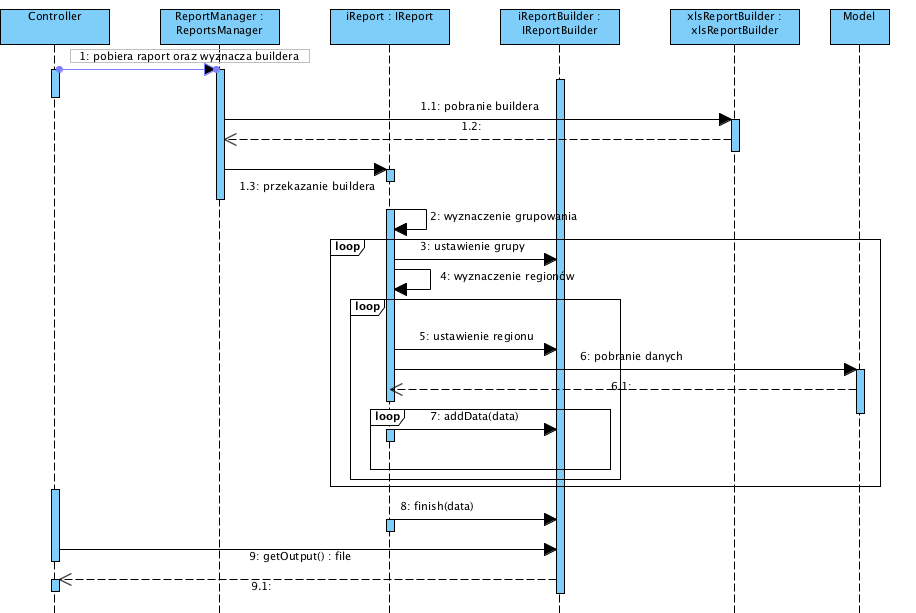
\includegraphics[width=15cm]{figures/image10}
\caption{Perspektywa procesu}\label{rys:use-case-diagram}
\end{figure}

Rysunek 5.10. wyjaśnia sposób przeprowadzenia komunikacji dotyczącej logowania do aplikacji, korzystając z zewnętrznego web service’u udostępnionego przez Politechnikę Poznańską. Przy próbie logowania użytkownik zostaje przekierowany na stronę Politechniki Poznańskiej, gdzie ma możliwość użycia danych logowania jednakowych dla wszystkich systemów Politechniki Poznańskiej. Po pomyślnym logowaniu otrzymuje token dostępu, wykorzystywany później do autoryzacji.

\begin{figure}[H] 
\centering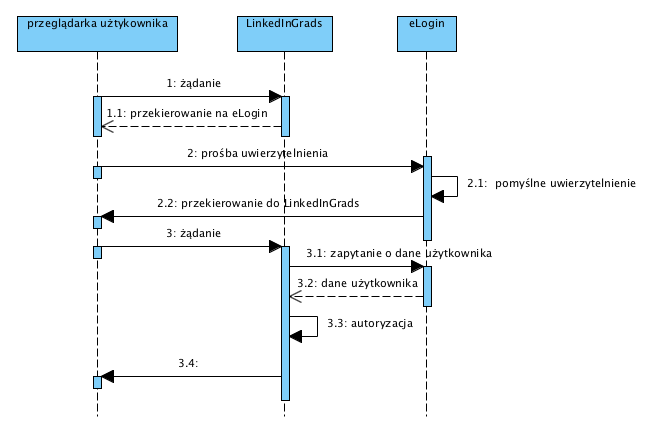
\includegraphics[width=15cm]{figures/image11}
\caption{Przepływ sterowania podczas uwierzytelnienia z systemem eLogin}\label{rys:use-case-diagram}
\end{figure}

\section{Decyzje projektowe i wybór technologii}

\subsection{DT1 Wybór platformy serwerowej Ruby on Rails}

Uzasadnienie: Platforma Ruby on Rails jest darmowa i dodatkowo posiada duże wsparcie społeczności, co skutkuje olbrzymią liczbą gotowych bibliotek, które można również za darmo wykorzystać. Ze względu na stosowane w niej `convention over configuration` przyjmuje rozsądne założenia dotyczące początkowej konfiguracji, co powoduje brak konieczności spędzania godzin na konfigurowaniu i przyspiesza rozpoczęcie właściwych prac. Framework ułatwia tworzenie aplikacji wykorzystujących wzorzec Model-View-Controller. Dodatkowo członkowie zespołu posiadają doświadczenie w tej technologii, co jest niewątpliwą zaletą.

\subsection{DT2 Wybór serwera HTTP Nginx oraz Phusion Passenger}

Uzasadnienie: Najpopularniejsze połączenie serwerowe używane przy serwowaniu aplikacji RubyOnRails, testowane przez setki użytkowników. Cechuje się dobrym wsparciem, łatwą i błyskawiczną konfiguracją oraz bardzo dobrą skalowalnością.

\subsection{DT3 Wybór systemu bazy danych PostgreSQL}

Uzasadnienie: System bazy danych wybrany został ze względu na zalecenia Działu Rozwoju Oprogramowania Politechniki Poznańskiej.

\subsection{DT4 Wybór technologii frontendowej Javascript oraz biblioteka jQuery}

Uzasadnienie: Wszechobecna technologia do tworzenia dynamicznych skryptów po stronie klienta, jest prosta w nauce i powszechnie znana przez programistów. Użycie biblioteki jQuery zdecydowanie upraszcza kod Javascript ułatwiając i przyspieszając m.in. manipulacje DOM.

\subsection{DT5 Wybór technologii backendowej gem pg oraz ActiveRecord}

Uzasadnienie: Biblioteka pg jest interfejsem relacyjnego systemu bazy danych PostgreSQL dla języka Ruby. Jest obecnie najchętniej używanym adapterem bazy danych, dlatego posiada bardzo dobre wsparcie jak i dokumentację.

ActiveRecord jest implementacją wzorca object-relational-mapping (ORM) i służy do mapowania relacyjnych baz danych na obiekty w języku Ruby. Minimalizuje to ilość kodu, która pozwala na stworzenie wiernego modelu obiektowego. Tak jak poprzednie rozwiązania, jest jednym z najpopularniejszych i wyznaje zasadę konwencji ponad konfiguracji. Charakteryzuje się m.in.:

\begin{itemize}
\item wygodnym sposobem modyfikacji schematu bazy danych przez migracje,
\item prostym tworzeniem (a także) rozszerzaniem walidacji oraz automatycznym wywoływaniem metod podczas różnych etapów życia obiektu,
\item banalną deklaracją relacji za pomocą zwykłych metod,
\item abstrakcją bazy danych poprzez użycie adapterów (np. wykorzystywany przez nas gem pg).
\end{itemize}

\subsection{DT6 Wybór technologii backendowej gem Savon}

Uzasadnienie: Biblioteka umożliwia połączenie z WebService’ami za pomocą protokołu SOAP. Najpowszechniej używany klient w języku ruby, znacząco upraszcza autoryzację użytkowników w systemie eLogin.

\subsection{DT7 Wybór technologii frontendowej LESS}

Uzasadnienie: Rozszerza kaskadowe arkusze styli o bardzo przydatne funkcje takie jak: 

\begin{itemize}
\item możliwość używania zmiennych, definiowania funkcji i wykonywania operacji
\item tworzenie `mixins`, które pozwalają na wielokrotne proste używanie zgrupowanych właściwości - klas styli - w różnych miejscach
\item wygodnej zagnieżdżonej składni, która zmniejsza objętość kodu i zwiększa jego czytelność
\end{itemize}	

Kompilowaniem LESS do CSS zajmuje się framework Rails, pozwala na to prosta konfiguracja gemem less-rails.

\subsection{DT8 Wybór technologii frontendowej HAML}

Uzasadnienie: HAML -  HTML abstraction markup language, silnik szablonów dla HTML. HAML wykorzystany został zamiast standardowego silnika szablonów jakim jest ERB. Charakteryzuje się m.in:

\begin{itemize}
\item prostotą, skrótowymi formami tworzenia tagów HTML - np. dokument HAML wykorzystuje wcięcia i rezygnuje z tagów zamykających,
\item wygodnym sposobem osadzania fragmentów kodu w języku Ruby w dokumencie HAML.
Powyższe powodują, że objętość kodu zmniejsza się drastycznie i dodatkowo zwiększa się jego czytelność ułatwiając tym samym wprowadzanie zmian.
\end{itemize}

\subsection{DT9 Wybór technologii frontendowej gem Spreadsheet}

Uzasadnienie: Biblioteka służąca do generowania plików formatu `.xls`

\section{Zależności między decyzjami projektowymi}

Rysunek 5.11. prezentuje zależności między decyzjami projektowymi. Linie obrazują możliwość podjęcia decyzji.

\begin{figure}[H] 
\centering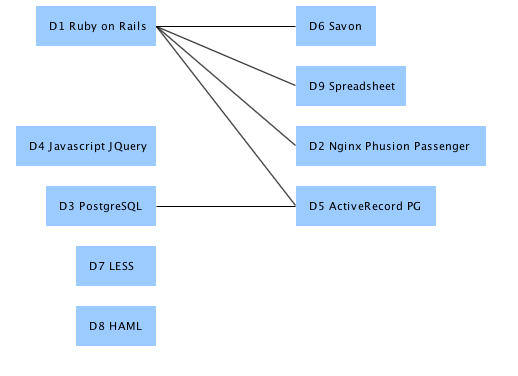
\includegraphics[width=15cm]{figures/image12}
\caption{Zależności decyzji projektowych}\label{rys:use-case-diagram}
\end{figure}

\section{Schemat bazy danych}

Rysunek 5.12. obrazuje relacje bazy danych w systemie LinkedInGrads.

\begin{figure}[H] 
\centering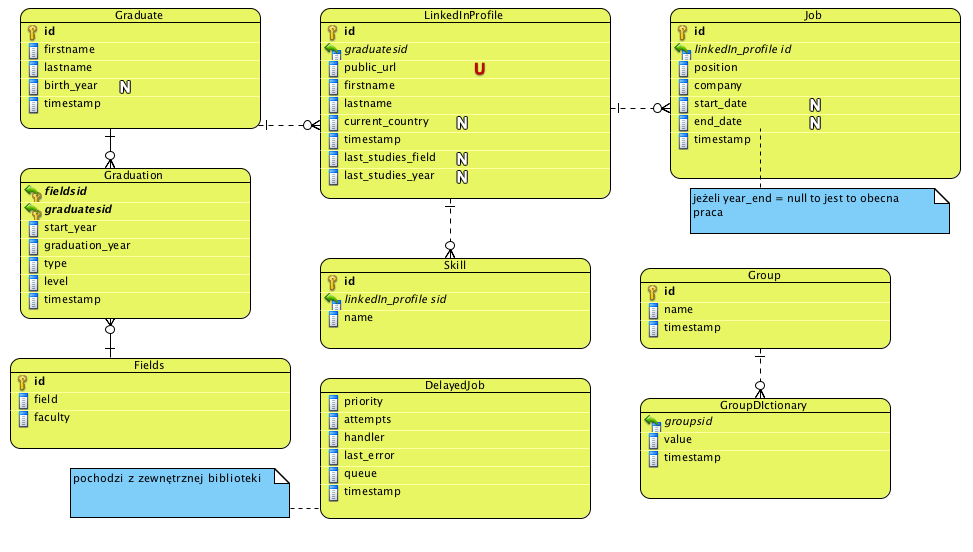
\includegraphics[width=15cm]{figures/image13}
\caption{Schemat bazy danych}\label{rys:use-case-diagram}
\end{figure}

Zastosowanie poszczególnych tabel:

\begin{itemize}
\item Graduate - tabela przechowująca informacje o absolwentach
\item Graduation - tabela przechowująca informacja o ukończonym profilu studiów
\item Field - tabela przechowująca metrykę profilu studiów
\item Skill - tabela przechowująca informacje o umiejętnościach absolwentów, pobieranych z serwisów zewnętrznych
\item LinkedInProfile - tabela przechowująca informacje o profilu absolwenta w serwisie zewnętrznym LinkedIn
\item Job - tabel przechowująca informacje o posadach obecnych i historycznych absolwentów, pobieranych z serwisów zewnętrznych
\item Group - tabela realizująca obiekt biznesowy Grupa opisany w podrozdziale 2.2.2
\item GroupDictionary - tabela 
\item DelayedJob - tabela tworzona przez zewnętrzną bibliotekę, odpowiadającą za wykonywanie zadań w tle
\end{itemize}